\begin{frame}[t]{Rýchlosť zmeny uhlov / orientácie}
\begin{itemize}
  \item<1-> Tvárme sa, že poznáme žiadanú uhlovú rýchlosť orientácie $r_{\dot{\Theta}}$, $r_{\dot{\Phi}}$ a $r_{\dot{\Psi}}$ a pre jednoduchosť sústredme len na rýchlosť zmeny klopenia ($\dot{\Theta}$).
  \item<2-> Sme na najnižšej úrovni, t.j. riadenie uhlovej rýchlosti \angl{rate controller} --- je to zároveň aj najdôležitejšia slučka, a máme 3 nezávislých slučiek \citep{AP:PID,PX4:PIDTuning}
  \item<3->  Je to aj najrýchlejšia slučka (cca. $f_s$=400--1000 Hz \citep{AP:PID,PX4:PIDTuning})
  \end{itemize}

  \begin{onlyenv}<1>
  \begin{figure}
\centering
  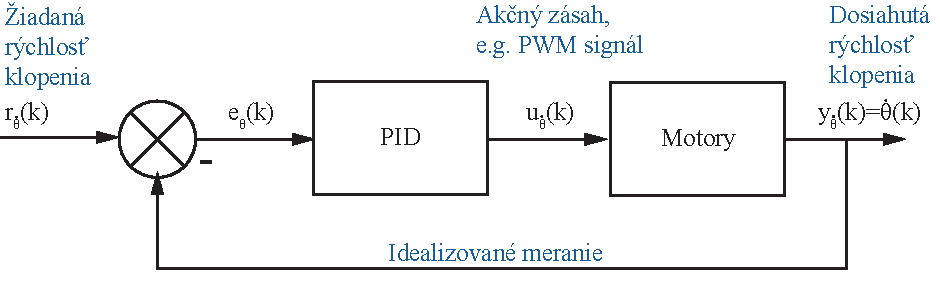
\includegraphics[width=\textwidth]{ATT_Rate}\\
\end{figure}
\end{onlyenv}

  \begin{onlyenv}<2-3>
  \begin{figure}
\centering
  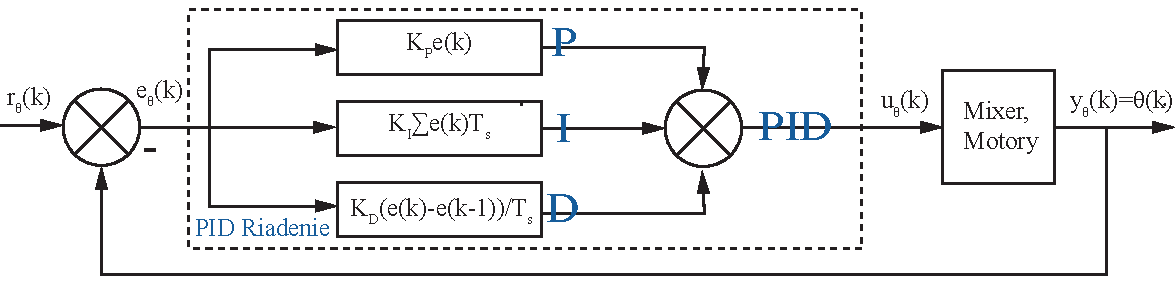
\includegraphics[width=\textwidth]{ATT_Rate2}\\
\end{figure}
\end{onlyenv}

  \end{frame}

\begin{frame}[t]{Ohraničenie vstupov}
  \begin{itemize}
    \item<1-> Akčné zásahy majú svoje ohraničenia (\angl{constraints})
    \item<2-> Ako donútime ich dodržanie? Saturáciou (orezávaním) hodnôt, ktoré skutočne vypočíta PID.
    \item<3-> Saturácia vnáša nelinearitu, vplýva na výkon riadenia aj stabilitu.
    \item<4-> Aj iné veličiny môžeme saturovať, napr. žiadané hodnoty. Ako by sme ohraničili výstup?
  \end{itemize}

    \begin{onlyenv}<2->
  \begin{figure}
\centering
  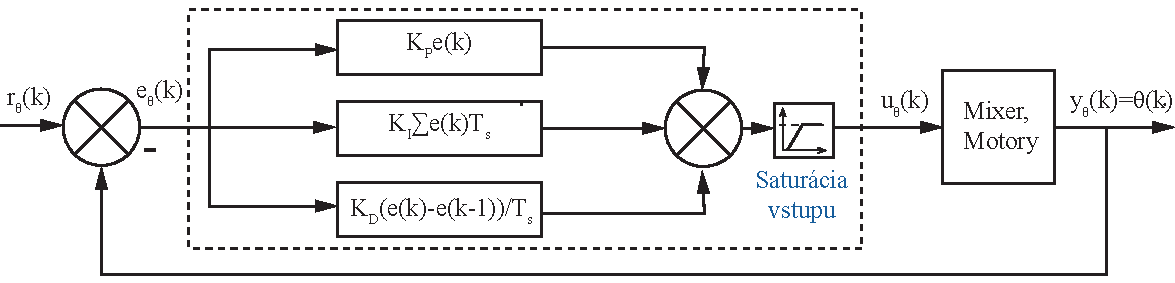
\includegraphics[width=\textwidth]{ATT_Rate3}\\
\end{figure}
\end{onlyenv}
\end{frame}


\begin{frame}[t]{Nahromadenie integračnej zložky}
  \begin{itemize}
    \item<1-> Integračná zložka ráta odchýlku v minulosti, preto ak akčné členy sú už na hraniciach možností - začína sa nahromaďovať \angl{windup}.
    %alebo sa to zbtočne nahromadí/začína sa zbytočne nahromaďovať (nemôže sa yačínať robiť sloveso v dokonavom vide...)
    \item<2-> Akonáhle sa vrátia akčné zásahy pod ohraničenia, nahromadená I zložka stále bude tlačiť systém na hranice možností, musí sa to chvíľu ``uvoľňovať'' \angl{unwind} a tým pádom prestrelíme \angl{overshoot} žiadané hodnoty
    \item<3-> To je saturácia integračnej zložky \angl{integral windup}.
    \item<4-> Môžeme používať rôzne triky, napr. ohraničiť veľkosť integračnej zložky, resp. vypnúť zložku pri určitých podmienkach.
  \end{itemize}
      \begin{onlyenv}<1-4>
  \begin{figure}
\centering
  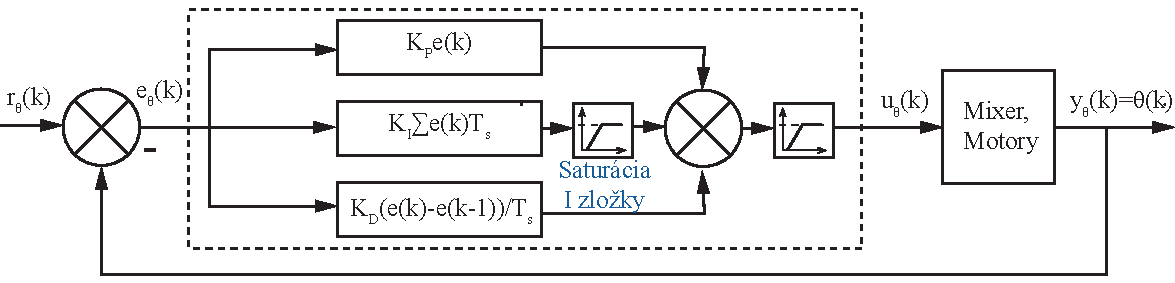
\includegraphics[width=\textwidth]{ATT_Rate4}\\
\end{figure}
\end{onlyenv}

      \begin{onlyenv}<5>
        \begin{itemize}
  \item<1-> ArduPilot - Ak akčný člen je akurát saturovaný, podrž hodnotu I zložky. Nižšie to môže ísť, vyššie nie \citep{AP:PID}.
  \item<2-> ArduPilot - Keďže máme kaskádnu konfiguráciu PID slučiek, saturačný znak postupuje cez hierarchiu nižšie a nižšie aby zastavil nahromadenie I zložky \citep{AP:PID}.
            \end{itemize}
      \end{onlyenv}

\end{frame}



\begin{frame}[t]{Šum a kopnutie derivačnej zložky}
  \begin{itemize}
    \item<1-2> Šum zo snímačov môže propagovať cez výpočet odchýlky riadenia do derivačnej zložky Vysokofrekvenčné zložky potom navýšia D zložku (čo je derivácia impulzu?)
    \item<2> Riešenie: Odchýlku riadenia pustíme cez dolnopriepustný \angl{low-pass} filter (LPF) --- Aj ArduCopter (20 Hz LPF) aj PX4 Autopilot používa \citep{AP:PID,PX4:PID}
    \item<3-> Náhle zmeny spôsobia ``kopnutie'' riadenia \angl{derivative kick}. (čo je derivácia impulzu?)
    \item<4-> Môžeme celkovo obísť zmenu žiadanej hodnoty a tým odchýlky  $e_\Theta(k)$ tak, že derivujeme výstup $y_\Theta(k)$\footnote{Riešenie v PX4, ArduCopter používa input shaping.}
  \end{itemize}
      \begin{onlyenv}<1-2>
  \begin{figure}
\centering
  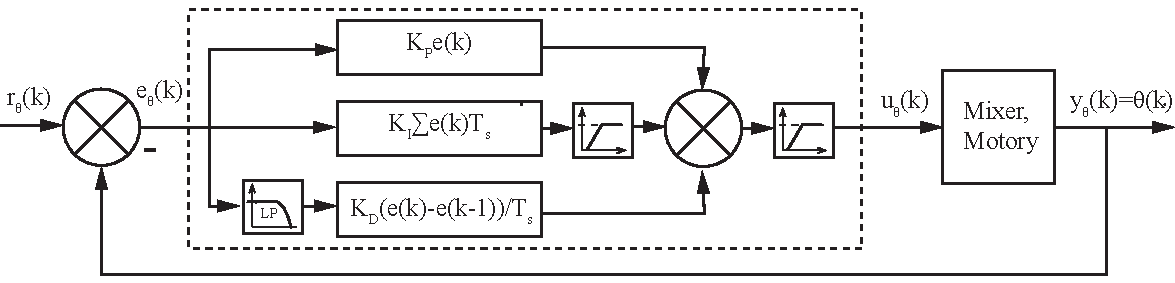
\includegraphics[width=\textwidth]{ATT_Rate5}\\
\end{figure}
\end{onlyenv}

\begin{onlyenv}<3->
  \begin{figure}
\centering
  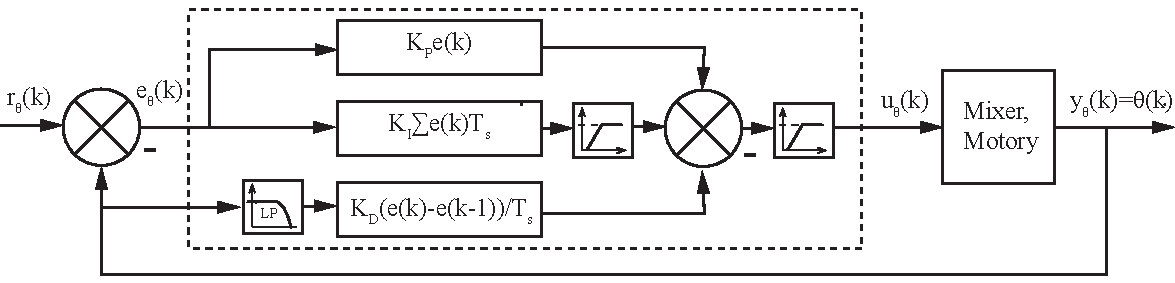
\includegraphics[width=\textwidth]{ATT_Rate6}\\
\end{figure}
\end{onlyenv}


\end{frame}

\begin{frame}{Ako to funguje v PX4?}
  \begin{figure}
\centering
  \includegraphics[width=100mm]{PX4_Rate}\\
\end{figure}

\end{frame} 